\documentclass[t, aspectratio=169]{beamer}
\usepackage[utf8]{inputenc}
\usepackage[T1]{fontenc}
\usepackage{amsthm,amsmath,amssymb}
\usepackage{tabularx}
\usepackage{booktabs}
\usepackage{array}
\usepackage[table]{xcolor}
\usepackage{lmodern}
\usepackage{graphicx}
\usepackage{tikz}
\usetikzlibrary{shapes.geometric, arrows.meta, positioning, calc}

% --- FONT SIZES ---
\setbeamerfont{frametitle}{size=\large}

% --- TIKZ STYLES ---
\tikzset{
    block_pink/.style={rectangle, draw, rounded corners, fill=pink!20, text width=3.5cm, text centered, minimum height=1.5cm},
    block_yellow/.style={rectangle, draw, rounded corners, fill=yellow!20, text width=3.5cm, text centered, minimum height=1.5cm},
    block_green/.style={rectangle, draw, rounded corners, fill=green!20, text width=3.5cm, text centered, minimum height=1.5cm},
    block_blue/.style={rectangle, draw, rounded corners, fill=blue!10, text width=3.5cm, text centered, minimum height=1.5cm},
    arrow/.style={-Latex, thick}
}

% --- MARGIN CONFIGURATION ---
\def\slideContentLeftMargin{0.5cm} 
\def\slideContentRightMargin{1cm}   
\def\hustHeaderHeight{1cm}        
\def\slideContentBotMargin{3.5cm}   

\usepackage[blue, 169]{beamerthemeHUST} 

\renewcommand{\titlePageTitleX}{-0.5cm}
\renewcommand{\titlePageTitleY}{-0.5cm}
\renewcommand{\hustTitleAlign}{\alignLeft} 
\renewcommand{\hustSubtitleAlign}{\alignLeft}
\renewcommand{\hustAuthorAlign}{\alignLeft}
\renewcommand{\hustInstAlign}{\alignLeft}

\title{IMPLEMENTATION OF PCB DEFECT DETECTION USING CUSTOM CNN ON TANG MEGA 138K PRO}
\author{\texorpdfstring{Nguyen Minh Sang \\ Nguyen Huu Son}{Nguyen Minh Sang, Nguyen Huu Son}} 
\institute{Viettel Manufacturing Coporation}

\begin{document}
	
	% Title page
	\husttitlepage
	
	\begin{frame}[allowframebreaks]{Table of Contents}
		\tableofcontents[hideallsubsections]
	\end{frame}
	
	\resetPageCount  
	\showPageNumber  
	
	\useStyleHustFull
	\useThinBar 
	
	% =================================================================
	\section{Introduction \& Objectives}
	% =================================================================
	
	\begin{frame}{Problem Statement}
		\textbf{Post-Soldering Automated Optical Inspection (AOI)}
		\begin{itemize}
			\item \textbf{Scenario (Post-Reflow):} After passing through the reflow soldering oven, Printed Circuit Boards (PCBs) must undergo strict quality inspection. The extreme heat can cause components to shift or fall off, and human/machine placement errors become permanently fixed.
			\item \textbf{Objective:} Develop a standalone FPGA-based vision system to rapidly detect \textbf{Missing Components} (fallen off during soldering) and \textbf{Reversed Polarity} (ICs/Capacitors soldered backward).
			\item \textbf{Standalone Execution:} Entire inference and post-processing pipeline must run on a single Tang Mega 138K Pro FPGA without relying on an external Host PC.
		\end{itemize}
	\end{frame}
	
	\begin{frame}{Technical Specifications \& Project Scope}
		\textbf{Target System Parameters for Tang Mega 138K Pro implementation:}
		
		\vspace{0.5em}
		\begin{itemize}
			\item \textbf{Vision \& Resolution Constraints:} 
            \begin{itemize}
                \item \textbf{Input Feed:} Single \textbf{1080p (1920$\times$1080) @ 30fps} MIPI CSI-2 stream.
                \item \textbf{ROI Processing:} Custom RTL Scaler dynamically crops bounding boxes and resizes them to \textbf{224$\times$224$\times$3} for CNN input.
                \item \textbf{Field of View (FOV):} Approx. \textbf{$100 \times 100$ mm} PCB capturing area.
                \item \textbf{Min. Component Size:} SMD \textbf{0603 / 0805} packages.
            \end{itemize}
            
			\item \textbf{AI \& Performance Parameters:} 
            \begin{itemize}
                \item \textbf{Inference Latency:} \textbf{$<50$ ms} per ROI ($\sim 20$ ROIs/second).
                \item \textbf{Model Size Limit:} \textbf{$< 1.5$ MB} (INT8 Quantized) to avoid BSRAM overflow.
                \item \textbf{Accuracy Target:} \textbf{$> 95\%$} on the validation set for 3 classes (OK, Missing, Reversed).
            \end{itemize}
            
            \item \textbf{Scope Limitation:} 
            \begin{itemize}
                \item \alert{\textit{Excluded:}} \textbf{Wrong component value} (requires macro-OCR).
            \end{itemize}
		\end{itemize}
	\end{frame}
	
	
	\begin{frame}{Physical System Layout}
		The proposed pipeline operates independently without requiring a PC.
		
		\vspace{0.5em}
		\begin{center}
		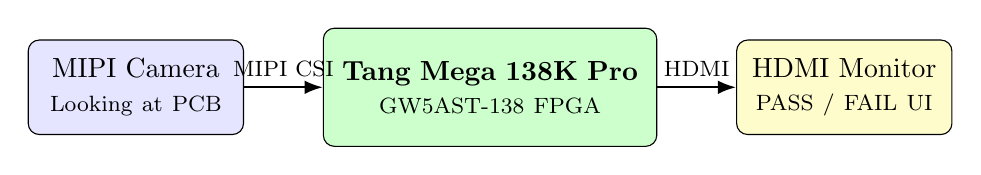
\begin{tikzpicture}[node distance=1cm and 1cm]
			\node (cam) [block_blue, text width=2.5cm, minimum height=1.2cm] {MIPI Camera \\ \footnotesize Looking at PCB};
			\node (fpga) [block_green, right=of cam, text width=4cm, minimum height=1.5cm] {\textbf{Tang Mega 138K Pro} \\ \footnotesize GW5AST-138 FPGA};
			\node (lcd) [block_yellow, right=of fpga, text width=2.5cm, minimum height=1.2cm] {HDMI Monitor \\ \footnotesize PASS / FAIL UI};
			
			\draw [arrow] (cam) -- node[above] {\footnotesize MIPI CSI} (fpga);
			\draw [arrow] (fpga) -- node[above] {\footnotesize HDMI} (lcd);
		\end{tikzpicture}
		\end{center}
		
		\vspace{0.5em}
		\begin{itemize}
			\item \textbf{Camera Module:} Mounted securely above the PCB alignment jig.
			\item \textbf{FPGA Kit:} Runs the standalone logic. Connected to a buzzer for auditory alarms.
			\item \textbf{Display:} Visualizes the PCB in real-time, overlaying color-coded boxes on inspected components.
		\end{itemize}
	\end{frame}
	
	% =================================================================
	\section{FPGA Standalone Architecture}
	% =================================================================
	\useStyleLogoOnly 
	\useThickBar      
	
	\begin{frame}{Proposed Standalone SoC Architecture}
		We propose a Heterogeneous System-on-Chip (SoC) based on the GoAI 3.0 SDK.
		
		\vspace{1em}
		\begin{center}
		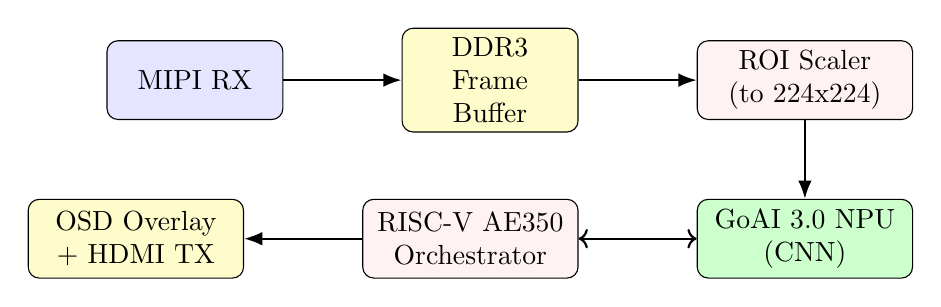
\begin{tikzpicture}[node distance=1cm and 1.5cm]
			\node (cam) [block_blue, text width=2cm, minimum height=1cm] {MIPI RX};
			\node (ddr) [block_yellow, right=of cam, text width=2cm, minimum height=1cm] {DDR3\\Frame Buffer};
			\node (scaler) [block_pink, right=of ddr, text width=2.5cm, minimum height=1cm] {ROI Scaler\\(to 224x224)};
			\node (npu) [block_green, below=of scaler, text width=2.5cm, minimum height=1cm] {GoAI 3.0 NPU\\(CNN)};
            \node (riscv) [block_pink, left=of npu, text width=2.5cm, minimum height=1cm] {RISC-V AE350\\Orchestrator};
            \node (osd) [block_yellow, left=of riscv, text width=2.5cm, minimum height=1cm] {OSD Overlay\\+ HDMI TX};
			
			\draw [arrow] (cam) -- (ddr);
			\draw [arrow] (ddr) -- (scaler);
			\draw [arrow] (scaler) -- (npu);
            \draw [arrow, <->] (riscv) -- (npu);
            \draw [arrow] (riscv) -- (osd);
		\end{tikzpicture}
		\end{center}
	\end{frame}
	
	\begin{frame}{Core Hardware System Components}
		\textbf{1. RISC-V Microcontroller (AE350):}
		\begin{itemize}
			\item Acts as the master orchestrator, iterating through a predefined \textbf{ROI List} (e.g., coordinates for R1, C1, U1).
			\item Coordinates the cropping, triggers inference, reads classification results, and raises GPIO alarms (Buzzer/LEDs) upon failure.
		\end{itemize}
		
		\vspace{1em}
		\textbf{2. Custom Hardware IPs (Verilog):}
		\begin{itemize}
			\item \textbf{ROI Scaler:} Crops the bounding box of a specific component from the 1080p frame buffer and resizes it to 224x224 on-the-fly.
			\item \textbf{GoAI 3.0 Accelerator:} Executes INT8 convolution layers.
            \item \textbf{OSD Overlay:} Hard-codes bounding boxes onto the HDMI output stream (Green = OK, Red = Missing, Yellow = Reversed).
		\end{itemize}
	\end{frame}
	
	\begin{frame}{Custom RTL Modules Architecture}
		To offload the RISC-V CPU and ensure real-time performance, we developed three custom Verilog modules:
		
		\vspace{0.5em}
		\begin{center}
		\resizebox{\textwidth}{!}{%
		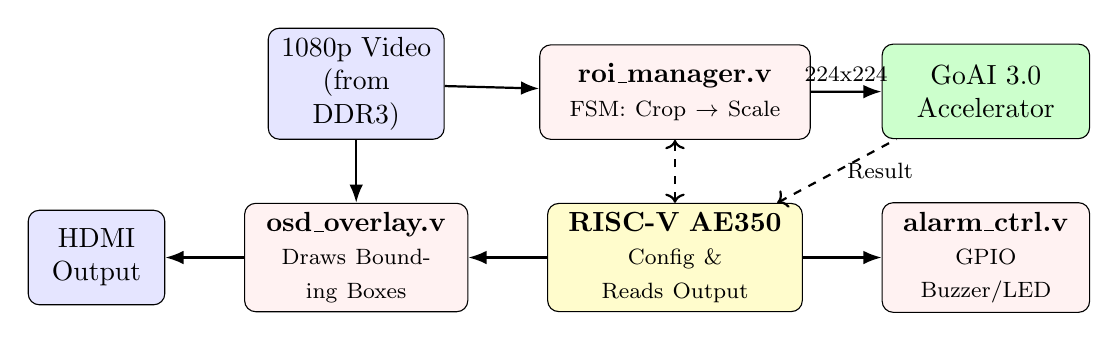
\begin{tikzpicture}[node distance=0.8cm and 1cm]
			% Bottom Row
			\node (osd) [block_pink, text width=2.6cm, minimum height=1.2cm] {\textbf{osd\_overlay.v}\\ \footnotesize Draws Bounding Boxes};
			
			\node (riscv) [block_yellow, right=of osd, text width=3cm, minimum height=1.2cm] {\textbf{RISC-V AE350}\\ \footnotesize Config \& Reads Output};
			
			\node (alarm) [block_pink, right=of riscv, text width=2.4cm, minimum height=1.2cm] {\textbf{alarm\_ctrl.v}\\ \footnotesize GPIO Buzzer/LED};
			
			\node (hdmi) [block_blue, left=of osd, text width=1.5cm, minimum height=1.2cm] {HDMI\\Output};
			
			% Top Row
			\node (vid_in) [block_blue, above=of osd, text width=2cm, minimum height=1.2cm] {1080p Video\\(from DDR3)};
			
			\node (roi) [block_pink, above=of riscv, text width=3.2cm, minimum height=1.2cm] {\textbf{roi\_manager.v}\\ \footnotesize FSM: Crop $\rightarrow$ Scale};
			
			\node (goai) [block_green, above=of alarm, text width=2.4cm, minimum height=1.2cm] {GoAI 3.0\\Accelerator};
			
			% Connections
			\draw [arrow] (vid_in) -- (roi);
			\draw [arrow] (roi) -- node[above]{\footnotesize 224x224} (goai);
			
			\draw [arrow, dashed, <->] (riscv) -- (roi);
			\draw [arrow, dashed, <-] (riscv) -- node[right]{\footnotesize Result} (goai);
			
			\draw [arrow] (riscv) -- (osd);
			\draw [arrow] (riscv) -- (alarm);
			
			\draw [arrow] (vid_in) -- (osd);
			\draw [arrow] (osd) -- (hdmi);
		\end{tikzpicture}%
		}
		\end{center}
	\end{frame}
	

	
    % =================================================================
	\section{AI Algorithm \& Training}
	% =================================================================
	\useStyleHustFull
	\useThinBar 
	
	\begin{frame}{Dataset \& Preprocessing}
		\begin{columns}[T] 
			
			\begin{column}{0.6\textwidth}
				\textbf{PCB Defect Dataset:}
				\begin{itemize}
					\item Custom-captured images of specific PCB components under identical lighting conditions.
					\item \textbf{Classes:} \texttt{OK}, \texttt{MISSING}, \texttt{REVERSED}.
                    \item Approximately 300-500 raw images per class.
				\end{itemize}
				
				\vspace{1em}
				\textbf{Data Augmentation:}
				\begin{itemize}
					\item Applying slight rotation, brightness variations, and shifting to increase robustness.
					\item Final dataset expanded to $\sim 1500$ images per class.
                    \item All inputs resized to $224 \times 224$ (RGB) to match the FPGA Scaler output.
				\end{itemize}
			\end{column}
			
			\begin{column}{0.4\textwidth}
				\begin{figure}
					\centering
                    % Placeholder for a PCB defect image
					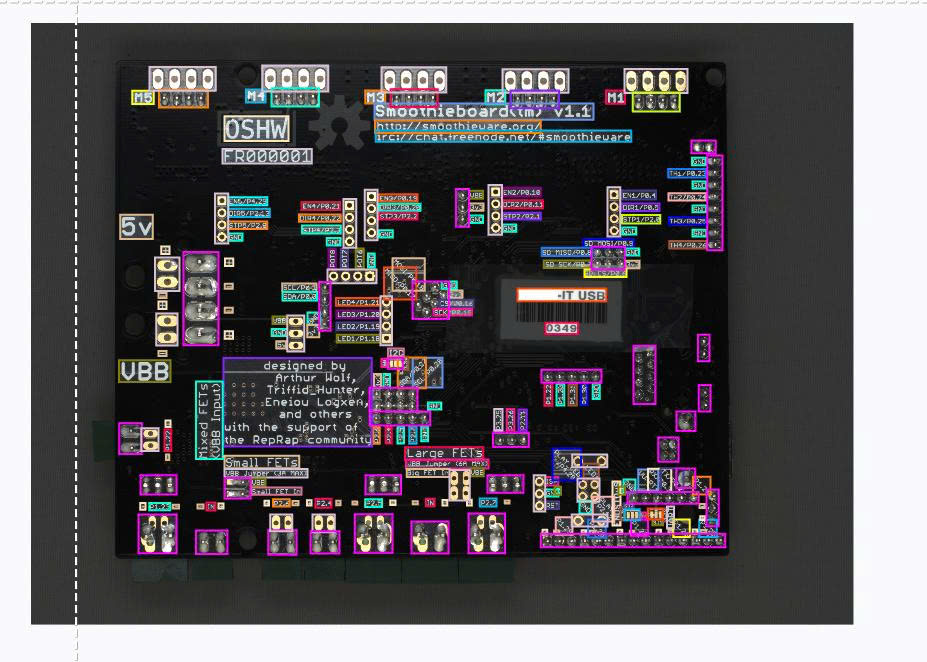
\includegraphics[height=5cm, keepaspectratio]{1785744785649_7010261324975782740_7010261324975782740_ffaa4d0efdf7ff239e27902b6d249830.jpg}
					\caption{Sample Dataset Variation}
				\end{figure}
			\end{column}
			
		\end{columns}
	\end{frame}
	
	\begin{frame}{Custom CNN Architecture for GoAI 3.0}
		We designed a lightweight CNN from scratch, strictly adhering to the operators supported by the GoAI 3.0 Hardware Accelerator.
		
		\vspace{1em}
		\begin{itemize}
			\item \textbf{Constraint:} The model \textbf{cannot} include unsupported operators like \texttt{BatchNorm} or \texttt{Dropout} in the exported graph.
		\end{itemize}
		
		\vspace{0.5em}
		\begin{center}
		\resizebox{\textwidth}{!}{%
		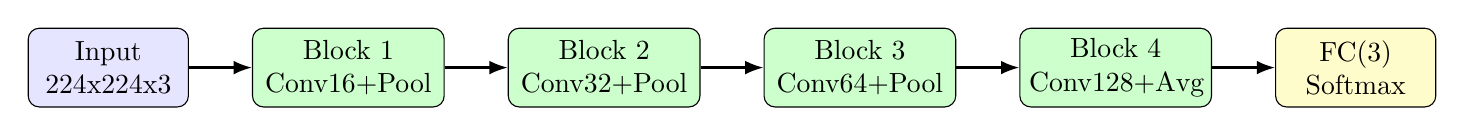
\begin{tikzpicture}[node distance=0.8cm and 0.8cm]
			\node (in) [block_blue, text width=1.8cm, minimum height=1cm] {Input\\224x224x3};
			\node (b1) [block_green, right=of in, text width=2.2cm, minimum height=1cm] {Block 1\\Conv16+Pool};
			\node (b2) [block_green, right=of b1, text width=2.2cm, minimum height=1cm] {Block 2\\Conv32+Pool};
			\node (b3) [block_green, right=of b2, text width=2.2cm, minimum height=1cm] {Block 3\\Conv64+Pool};
			\node (b4) [block_green, right=of b3, text width=2.2cm, minimum height=1cm] {Block 4\\Conv128+Avg};
			\node (out) [block_yellow, right=of b4, text width=1.8cm, minimum height=1cm] {FC(3)\\Softmax};
			
			\draw [arrow] (in) -- (b1);
			\draw [arrow] (b1) -- (b2);
			\draw [arrow] (b2) -- (b3);
			\draw [arrow] (b3) -- (b4);
			\draw [arrow] (b4) -- (out);
		\end{tikzpicture}%
		}
		\end{center}
		
		\begin{itemize}
			\item \textbf{Result:} A highly efficient classifier specifically tuned for the NPU.
		\end{itemize}
	\end{frame}
	
	\useStyleLogoOnly 
	\useThickBar 

	\begin{frame}{Training \& Quantization Pipeline}
		The model must be quantized to INT8 before hardware deployment.
		
		\vspace{1.5em}
		\begin{center}
		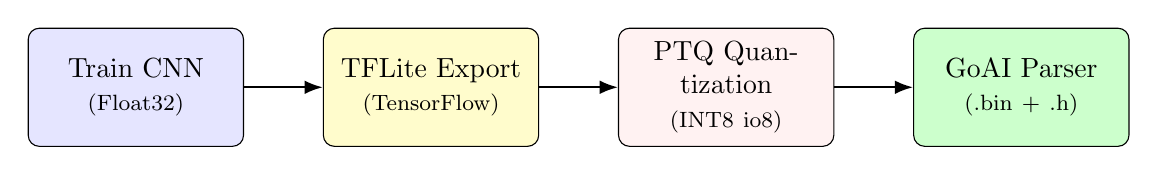
\begin{tikzpicture}[node distance=1cm and 1cm]
			\node (train) [block_blue, text width=2.5cm] {Train CNN \\ \footnotesize (Float32)};
			\node (export) [block_yellow, right=of train, text width=2.5cm] {TFLite Export \\ \footnotesize (TensorFlow)};
			\node (quant) [block_pink, right=of export, text width=2.5cm] {PTQ Quantization \\ \footnotesize (INT8 io8)};
            \node (header) [block_green, right=of quant, text width=2.5cm] {GoAI Parser \\ \footnotesize (.bin + .h)};
			
			\draw [arrow] (train) -- (export);
			\draw [arrow] (export) -- (quant);
            \draw [arrow] (quant) -- (header);
		\end{tikzpicture}
		\end{center}
        
        \vspace{1em}
        \textbf{Full Integer Quantization:}
        \begin{itemize}
            \item We utilized a representative dataset to calibrate activation ranges.
            \item Enforced INT8 input/output (\texttt{io8}) to ensure seamless integration with the GoAI C-firmware without requiring floating-point conversions on the RISC-V.
        \end{itemize}
	\end{frame}
	


    % =================================================================
	\section{Development Roadmap}
	% =================================================================
	\useStyleLogoOnly 
	\useThickBar 

\begin{frame}{Development Roadmap (13-Week Plan)}
\vspace{0.5em}
\begin{center}
\resizebox{0.95\textwidth}{!}{%
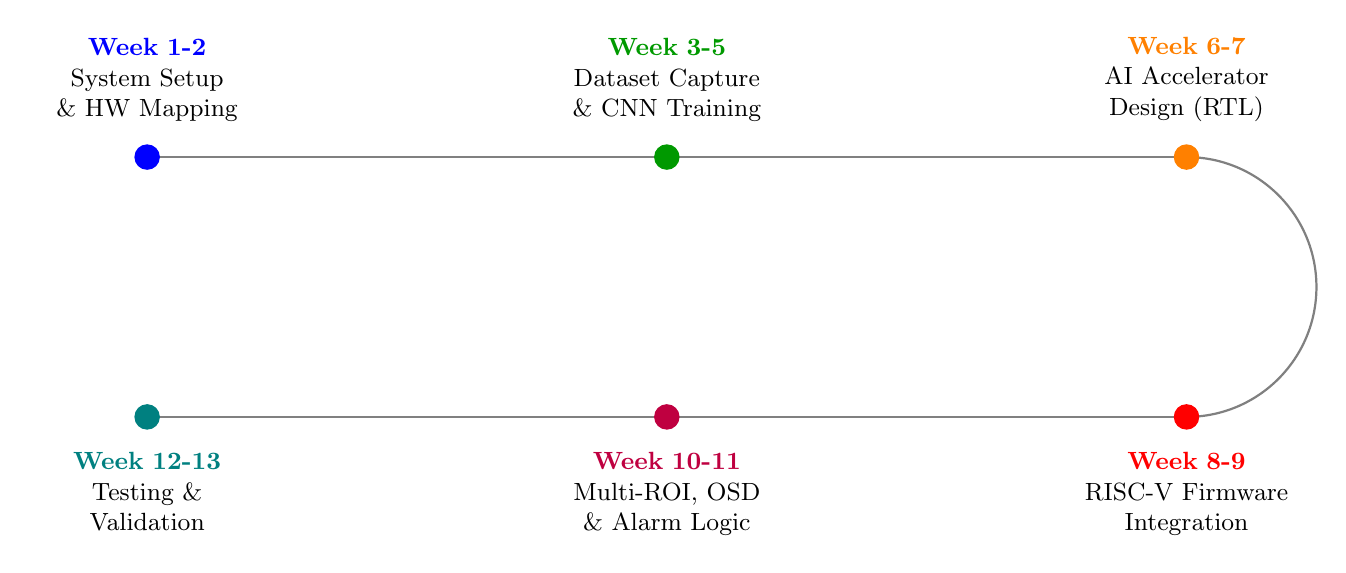
\begin{tikzpicture}[scale=1.1]

    % Lines
    \draw[thick, gray] (0,0) -- (12,0);
    \draw[thick, gray] (12,0) arc (90:-90:1.5cm);
    \draw[thick, gray] (12,-3) -- (0,-3);

    % Points - Top
    \filldraw[blue] (0,0) circle (4pt);
    \filldraw[green!60!black] (6,0) circle (4pt);
    \filldraw[orange] (12,0) circle (4pt);

    % Points - Bottom
    \filldraw[red] (12,-3) circle (4pt);
    \filldraw[purple] (6,-3) circle (4pt);
    \filldraw[teal] (0,-3) circle (4pt);

    % Labels Top (smaller + narrower)
    \node[anchor=south, text width=2.8cm, align=center, font=\small]
    at (0,0.3)
    {\textcolor{blue}{\textbf{Week 1-2}}\\System Setup\\\& HW Mapping};

    \node[anchor=south, text width=2.8cm, align=center, font=\small]
    at (6,0.3)
    {\textcolor{green!60!black}{\textbf{Week 3-5}}\\Dataset Capture\\\& CNN Training};

    \node[anchor=south, text width=2.8cm, align=center, font=\small]
    at (12,0.3)
    {\textcolor{orange}{\textbf{Week 6-7}}\\AI Accelerator\\Design (RTL)};

    % Labels Bottom
    \node[anchor=north, text width=2.8cm, align=center, font=\small]
    at (12,-3.3)
    {\textcolor{red}{\textbf{Week 8-9}}\\RISC-V Firmware\\Integration};

    \node[anchor=north, text width=2.8cm, align=center, font=\small]
    at (6,-3.3)
    {\textcolor{purple}{\textbf{Week 10-11}}\\Multi-ROI, OSD\\\& Alarm Logic};

    \node[anchor=north, text width=2.8cm, align=center, font=\small]
    at (0,-3.3)
    {\textcolor{teal}{\textbf{Week 12-13}}\\Testing \& Validation};

\end{tikzpicture}
}
\end{center}
\end{frame}

    \begin{frame}{Hardware Requirements \& Preparation}
		To successfully implement the standalone AOI pipeline, the following hardware components are required:
		
		\vspace{1em}
		\begin{enumerate}
			\item \textbf{Processing Core (Available):} Tang Mega 138K Pro FPGA Kit (GW5AST-138).
			\item \textbf{Vision Input:} 
            \begin{itemize}
                \item MIPI CSI-2 Camera Module (e.g., OV5640 5MP or IMX219 8MP).
                \item \textbf{Macro Lens:} Essential for close-up focusing on tiny 0402/0603 SMDs without blur.
            \end{itemize}
            \vspace{0.3em}
			\item \textbf{Display Output:} Standard HDMI Monitor and cable for the Real-time OSD Pass/Fail Interface.
            \vspace{0.3em}
            \item \textbf{Illumination:} Industrial Ring Light (LED) or shadowless diffused lighting to prevent glare from solder joints.
            \vspace{0.3em}
            \item \textbf{Mechanical Setup:} A stable Camera Stand and a PCB Alignment Jig to keep the testing board perfectly static during single-frame capture.
		\end{enumerate}
	\end{frame}

    % =================================================================
	\section{Future Works}
	% =================================================================
	\useStyleLogoOnly 
	\useThickBar 

    \begin{frame}{Future Works}
		\begin{enumerate}
            \item \textbf{Recognizing Component Values (OCR):} 
            \begin{itemize}
                \item Add an Optical Character Recognition (OCR) model to read printed text on tiny resistors, enabling the system to detect "Wrong Value" defects.
            \end{itemize}
            
            \vspace{0.8em}
            \item \textbf{Automating ROI Generation from Gerber Files:} 
            \begin{itemize}
                \item Currently, component coordinates (bounding boxes) are coded manually.
                \item We plan to build a software that reads standard PCB Gerber files and automatically generates the coordinate array for the FPGA.
            \end{itemize}
            
            \vspace{0.8em}
            \item \textbf{Smart Factory Integration (IoT):} 
            \begin{itemize}
                \item Integrate Ethernet/WiFi modules to transmit real-time defect logs directly to the factory's management server (MES).
            \end{itemize}
        \end{enumerate}
	\end{frame}

	\hustthankyou
	
\end{document}